\subsection{Сформулировать квантовомеханическую задачу для гармонического осциллятора. Получить
его решение. Указать, на каком этапе решения возникает квантование энергии. Правила отбора
для гармонического осциллятора.}
Рассмотрим гармонические колебания в одномерном случае. В классической физике
имеем\footnote{Понятно, что в реальности такой силы сущестовать не может и
рассмотрение ограничивается приближёнными малыми колебаниями.} $ F_x = -kx $, и, значит,  
\begin{equation}
    U(x) = \frac{kx^2}{2} = \frac{m_0\omega_0^2 x^2}{2},
    \label{eq:potenc}
\end{equation}
где $ \omega_0^2 = k/m_0 $ --- квадрат собственной частоты классического
гармонического осцилятора. Таким образом, рассматривается движение частицы в
параболической потенциальной яме. 
\begin{figure}[h]
  \centering
  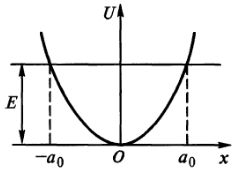
\includegraphics[width=0.3\textwidth]{img/write-02/yama.png}
  \caption{Потенциальная энергия гармонического осциллятора.}
  \label{fig:yama}
\end{figure}
На рисунке \ref{fig:yama} число $ a_0 $ есть, конечно,
амплитуда колебаний. Считая без потери общности движение равным $ x = a_0 \cos\omega t $, легко
получим 
\[
    E = \frac{m_0a_0^2\omega_0^2}{2}, \quad a_0 =
    \sqrt{\frac{2E}{m_0\omega_0^2}}.
\]

Перейдём к квантовому случаю. А именно, решим уравнение Шрёдингера
для потенциальной энергии \eqref{eq:potenc}: 
\[
    \frac{\hbar^2}{2m} \psi''(x) + \left(E - \frac{kx^2}{2}\right) \psi(x) = 0.
\]

\subsubsection{Решение уравнения}
\textbf{1. Масштабирование}. Перейдём к безразмерным величинам $ \varepsilon =
E/E_0 $, $ \xi = x/x_0 $. Здесь $ E_0 = E_{\min} = \hbar \omega/2 = kx_0/2 $.
Обоснуем: 
\begin{align*}
  \Delta x &= \sqrt{\langle x^2\rangle} = \sqrt{\frac{1}{2} a_0^2} =
  \sqrt{\frac{E}{m_0\omega_0^2}},\\
  \Delta p &= \sqrt{\langle p^2 \rangle} =
  \sqrt{\frac{1}{2}m_0^2a_0^2\omega_0^2} = \sqrt{m_0E},
\end{align*}
откуда вместе с неравенством Гейзенберга $ \Delta x \Delta p \geqslant \hbar/2 $
и следует результат. Итак, перейдём к величинам $ \varepsilon $, $ \xi $ и
получим уравнение
\begin{equation}
  \psi'' + (\varepsilon - \xi^2)\psi = 0.  
  \label{eq:eq1}
\end{equation}

\textbf{2. Асимптотика.} Устремим в уравнении $ |\xi| \to \infty $. Тогда
главная часть примет вид 
\[
    \psi'' = \xi^2 \psi.
\]
Согласно граничным условиям\footnote{См. первый постулат. Мы ищем регулярные
  решения, то есть такие, интеграл квадрата которых сходится, откуда и получаем
указанное условие.} $ \psi \to 0 $, откуда вытекает предположение о виде волновой функции
$ \psi = e^{\alpha(\xi)} $, где $ \alpha(\xi) \to -\infty $. Тогда $ \psi'' =
(\alpha'' + (\alpha')^2)e^\alpha $, а значит, $ \alpha'' + (\alpha') = \xi^2 $.
Тогда (?) $ \alpha = A\xi^n $. В этом предположении в связи с рассматриваемой
асимптотикой будем рассматривать только слагаемое в квадрате, получим $
A^2n^2\xi^{2n-2} \approx \xi^2 $, откуда $ A = -1/2 $, $ n= 2 $. Искомая
асимптотика --- $ \psi  \to \exp( - \xi^2/2) $.

\textbf{3. Общий вид.} Будем в таком случае искать решение в виде $ \psi(\xi) =
\exp(-\xi^2/2)f(\xi)$. Подставив в \eqref{eq:eq1} и упростив выражение, получим 
\begin{gather*}
    \psi'' = \exp(-\xi^2/2)^{(2)}f + 2\exp(-\xi^2/2)^{(1)}f^{(1)} +
    \exp(-\xi^2/2) f^{(2)} = \exp(-\xi^2/2)(f''-2\xi f' + (\xi^2 - 1)f),\\
    f'' - 2\xi f' + (\varepsilon - 1)f = 0.
\end{gather*}
Саму функцию $ f $ представим рядом $ f = \sum\limits_{k=0}^{\infty} a_k
\xi^k$. Тогда  
\begin{align*}
  f' &= \sum_{k=0}^\infty ka_k \xi^{k-1},\\
  f'' &= \sum_{k=0}^\infty k(k-1) a_k
  \xi^{k-2} = \sum_{k=0}^\infty (k+1)(k+2) a_{k+2}\xi^k.
\end{align*}
Получаем для любого $ \xi $  
\[
  \sum_{k=0}^\infty ((k+2)(k+1)a_{k+2} + (-2k + \varepsilon - 1) a_k)\xi^k = 0.
\]
Благодаря произвольности $ \xi $ можем вывести теперь рекуррентное соотношение 
\begin{equation}
  a_{k+2} = \frac{2k+1-\varepsilon}{(k+2)(k+1)}a_k \approx \frac{2}{k}a_k
  \label{eq:rek}
\end{equation}
при $ k \to \infty $. С другой стороны для некоторого $ k' = k/2 $
\[
  \exp(\xi^2) = \sum_{k'=0}^\infty \frac{\xi^{2k'}}{k'!} = \sum_{k=0}^\infty
  \frac{\xi^k}{(k/2)!},
\]
где для последнего ряда также выполняется предельное рекуррентное соотношение
\eqref{eq:rek}. Поэтому и примем $ f(\xi) = \exp(\xi^2) $. Однако в этом случае
$ \psi = \exp(\xi^2/2) \to \infty $ при $ \xi \to \infty $.

\textbf{4. Квантование.} Приходим к тому, что ряд $ f(\xi) $ нужно оборвать.
Рассмотрим индекс последнего ненулевого члена $ n := k_{\max} $ и нулевой член $ a_{n+2} $. Из реккурентного
соотношения \eqref{eq:rek} вытекает теперь, что $ \varepsilon = 2n+1 $. Заметим,
что этот факт и говорит о квантовании энергии. Сама энергия имеет вид
\[
  E_n =
  \frac{\hbar \omega_0}{2} + n\hbar\omega_0.
\]

\textbf{5. Полиномы Чебышёва -- Эрмита.} Получили, что $ f(\xi) $ есть некие
полиномы степени $ n $. Конкретный вид полиномов выберем из соображений
ортогональности решений. Ими будут полиномы Эрмита  
\[
  H_n := (-1)^n \exp(x^2) \frac{d^n}{d\xi^n}\exp(-x^2),
\]
которые как раз имеют
\emph{вес} $ \exp(-\xi^2) $, то есть 
\[
  \int\limits_{-\infty}^{\infty}H_n H_m \exp(-\xi^2)\,d\xi =
  \frac{\delta_{nm}}{A_nA_m},
\]
где коэффициент 
\[
  A_k = \frac{1}{\sqrt{2^kk!\sqrt{\pi}}}.
\]

Таким образом, волновые функции будут равны 
\[
    \psi_n(\xi) = A_n \exp(-x^2/2) H_n(\xi).
\]
\qed

\begin{figure}[h]
  \centering
  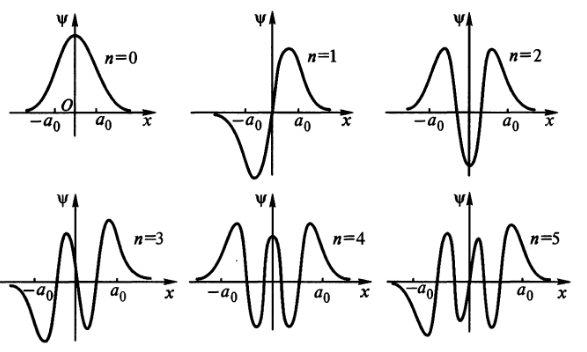
\includegraphics[width=0.8\textwidth]{img/write-02/psi.png}
  \caption{Волновые функции гармонического осциллятора}
  \label{fig:psi}
\end{figure}

Обратим внимание, что энергия, а значит, амплитуда $ a_0 $ зависят от $ n $. При
этом в отличие от прямоугольных ям энергия с переходом на новый уровень меняется
на равные отрезки $ \Delta E = \hbar\omega_0 $. Точный расчет
показывает, что особенности испускания и поглощения 
электромагнитного излучения гармоническим осциллятором таковы, что 
возможны переходы только между соседними уровнями. Условия, которые определяют
изменение квантовых чисел при разрешенных переходах системы из одного состояния в другое,
называются правилами отбора. Таким образом, согласно правилам
отбора, квантовое число $ n $ при испускании и поглощении 
электромагнитного излучения квантовым гармоническим осциллятором
может изменяться только на единицу.

Снова минимальная энергия положительна, что играет очень важную роль в физике (см., напр.,
отсутствие кристаллизация гелия при абсолютном нуле и нормальном давлении).

Попробуем рассчитать вероятность для классического осциллятора. Там $ x =
a_0\sin \frac{2\pi}{T}t $, $ dx = a_0 \frac{2\pi}{T} \cos \frac{2\pi}{T}t\,dt $,
и вероятность $ dP $ того, что
частица при движении в одну сторону находится в интервале шириной $ dx $,
равна 
\[
  dP = \frac{dt}{T/2} = \frac{dx}{\pi\sqrt{a_0^2 - x^2}}.
\]
При больших $ n $ функция $ |\psi_n|^2 $ похожа на $ dP/dx $, однако для малых
$ n $ они отличаются очень сильно.

\begin{figure}[h]
  \centering
  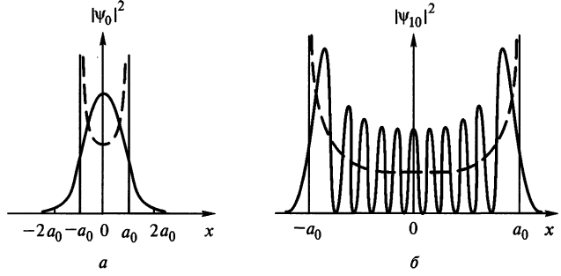
\includegraphics[width=0.8\textwidth]{img/write-02/dPdx.png}
  \caption{Плотности вероятности обнаружения частицы для 
квантового (сплошная линия) и классического (пунктирная линия) осциллятора.}
  \label{fig:dPdx}
\end{figure}
